\chapter{Introduction}
% \minitoc
% \printMarginPartialToc
As the year went on, I started typesetting my personal notes during class and realized that the \LaTeX  format, 
while great for publications and lecture notes in general, was lacking a few small but useful template for me.

\section{Required Packages}\label{sec:reqpackages}
For \textit{Subook,} the following packages are required
\begin{center}
    \texttt{marginnote, sidenotes, fancyhdr, titlesec, geometry, and tcolorbox.}
\end{center}
For a brief summary, the \texttt{marginnote}, \texttt{sidenote}, \texttt{titlesec}, 
and \texttt{tcolorbox} packages are used in creating the \texttt{$\backslash$part} environment, 
the package \texttt{geometry} is used globally to set the page width, page height, 
and margin width, and finally, \texttt{fancyhdr}, 
which is overridden on the title page, 
the contents page, and the \texttt{$\backslash$part} page, sets the header for the body.


\section{License}\label{sec:license}
This work may be distributed and/or modified under the conditions of the LaTeX Project Public License, 
either version 1.3 of this license or (at your option) any later version. 
The latest version of this license is found in  \url{http://www.latex-project.org/lppl.txt}, 
and version 1.3 or later is part of all distributions of LaTeX version 2005/12/01 or later. 
The current maintainer of this work is Changxing Su.

\section{Features}\label{sec:Features}

\textit{Subook} includes the following:
	\begin{enumerate}
		\item Several mathematics and physics packages.
		\item Margins and margin environments for tables, figures, and asides.
		\item \TeX\ shortcuts for various math scripts namely vector bold math, \texttt{mathbb}, \texttt{mathfrak}, and \texttt{mathcal}.
		\item \texttt{amsthm} integrations and special environments for theorems, lemmas, proofs, definitions, examples, and remarks.\
		\item Stylized support for the \texttt{part} environment.
		\item A fullpage environment that spans across the text width and the margin for longer equations and horizontal figures.
	\end{enumerate}
    Each of these will be discussed in the following subsections.


\section{\TeX\ Shortcuts}\label{sec:shortcuts}
\textit{subook} comes built in with a minimal set of keyboard shortcuts for a few special characters. All of these shortcuts can be found in \texttt{subook.cls} just under
\begin{verbatim}
% ----------------------------------------------------------------------
%           User Created Commands
% ----------------------------------------------------------------------
...
\end{verbatim}
If one has their own macros\mn{Most people have their own shortcuts for commonly used mathematics, such as derivatives or integrals. For those looking for physics shortcuts, the {excellent} \texttt{physics} package (automatically included in \textit{subook}) has possible everything that one can imagine.} then simply add it under this area. 


\section{\texttt{amsthm} Environments}\label{Sub:Special}
\texttt{amsthm} environments are defined as usual being enclosed by \texttt{$\backslash$begin\{environment\}}$\cdots$ \texttt{$\backslash$end\{environment\}} 
and most have been modified ostensibly from the original \texttt{amsthm} presets. 
Primarily, most environments, 
with the exception of the exercise environment, are now integrated with the wonderful \texttt{tcolorbox} package. 
Note that the counting for \texttt{theorems} and \texttt{lemmas} is distinct from the counting for \texttt{definitions}. 
Also note that the \texttt{breakable} for \texttt{tcolorbox} allows these environments to span multiple pages.
All of these environment and the associated \texttt{tcolorbox} are provided by the  code in \texttt{subook.cls} just under \lecture.
\begin{verbatim}
    % ----------------------------------------------------------------------
    %                         User Created Environments 
    % ----------------------------------------------------------------------
    ...
    %% ------------------------------ tcolorbox  ---------------------------
    ...
\end{verbatim}

\begin{definition}[Test]
    The \texttt{definition} environment
\end{definition}


\begin{lemma}[Test]
    The \texttt{lemma} environment
\end{lemma}

\begin{theorem}[Test]
    The \texttt{theorem} environment
\end{theorem}

\begin{corollary}[Test]
    The \texttt{corollary} environment
\end{corollary}

\begin{proposition}[Test]
    The \texttt{proposition} environment
\end{proposition}


\begin{example}[Test]
    The \texttt{example} environment
\end{example}

\begin{proof}
    The \texttt{proof} environment
\end{proof}


\begin{remark}
    The \texttt{remark} environment
\end{remark}

\begin{assumption}
asdasd
\end{assumption}

\begin{exercise}
sdadsa
\end{exercise}
\begin{tbox}{Some extra box environment}
    The \texttt{something extra} environment
\end{tbox}

% \begin{examplebox}{Test}
%     I use my ``examplebox'' as usual text and margin figure work as they should be but I want my example box spread out to the right margin on an odd page, breakable, and spread out to the left margin on the even page.
%     \tcblower
%     I use my ``examplebox'' as usual text and margin figure work as they should be but I want my example box spread out to the right margin on an odd page, breakable, and spread out to the left margin on the even page.
% \end{examplebox}

\subsection{\texttt{tcolorbox} Environment and Known Issues}
\label{ssub:tcolorbox environments_and_known_issues}


The \texttt{breakable} should allow the \texttt{proof} environment to span multiple pages. If one wishes to change the color, simply modify the line which states \texttt{borderline west=\{1pt\}} \texttt{\{0pt\}\{blue\}}. The first numeric value dictates the width of the line, the second dictates how close it is away from the \textit{left} margin, while the last argument obviously dictates the color. This code could also be used to change any of the other \texttt{amsthm} environments
\marginpar{
    \centering
    \includegraphics[width=0.4\textwidth]{example-image-a}
    \captionof{figure}{marginfigure}}.


\section{Fullpage Environment}\label{Sec: Fullpage}

\begin{fullpage}
    The \texttt{fullpage} environment is defined by
    \begin{center}
        \texttt{$\backslash$begin\{fullpage\}}\\
        $\cdots$\\
        \texttt{$\backslash$end\{fullpage\}}
    \end{center}
    with the width of the \texttt{fullpage} environment given by \texttt{$\backslash$textwidth}+\texttt{$\backslash$marginparsep}+\texttt{$\backslash$marginparwidth}
    There are some clear benefits of having use of the full page at times. Suppose that one wants to place a figure that cannot fit into the margins, or if an equation is quite long and it bleeds into
     the margin, 
    then the \texttt{fullpage} environment can both clearly separate these from the surrounding text and allot for the dimensions without hassle. 
%% //FIXME  : When using figure enviorment, recipe terminated with error by message"Float(s) lost." 
    % \begin{figure}

    \centering
        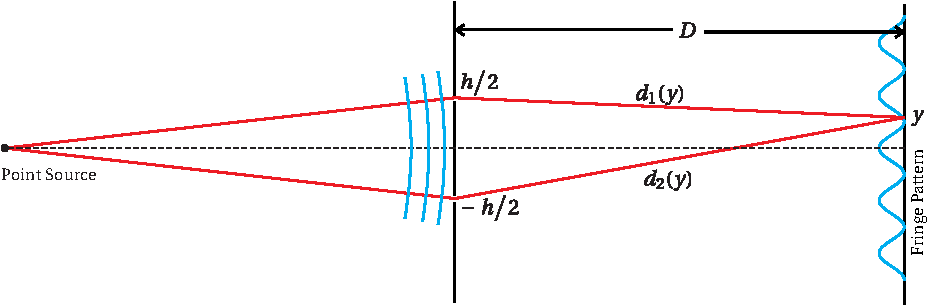
\includegraphics{img/f08Young.pdf}
        \captionof{figure}{Figure caption}
        \label{fig:example} % Unique label used for referencing the figure in-text
    %     %\addcontentsline{toc}{figure}{Figure \ref{fig:placeholder}} % Uncomment to add the figure to the table of contents
    % \end{figure}
    \begin{definition}[big box]
        dsdd
    \end{definition}
\end{fullpage}

\texttt{Figure} is a floating environment and \texttt{minipage} is, unfortunately, not. Therefore, if you put a floating object inside a non-floating minipage, you will get an error.One way is to avoid using figure entirely. This can be done with help of the caption package (with its captionof facility, so that you can have a caption for the figure):
%% solution from https://tex.stackexchange.com/questions/55337/how-to-use-figure-inside-a-minipage
\begin{lstlisting}
    \centering
        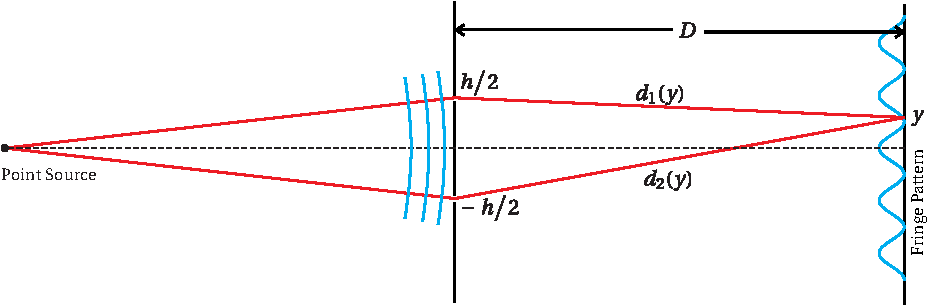
\includegraphics{img/f08Young.pdf}
        \captionof{figure}{Figure caption}
        \label{fig:example} % Unique label used for referencing the figure 
\end{lstlisting}
Table\marginpar{\centering
\begin{tabular}{lll}
\toprule
1 & 1 & 1\\
\midrule
1 & 1 & 0.562 \\
2 & 1 & 0.910 \\
3 & 11 & 0.296 \\
\bottomrule
\end{tabular}
\captionof{table}{Sophisticated margin table}
}The genomes of chimpanzees and humans are 99.9\% identical, yet the differences between the two species are vast. The relatively few differences in genetic endowment must explain \marginpar[right]{dsdsdsdsd}the possession of language by humans, the extraordinary athleticism of chimpanzees, and myriad other differences. Genomic comparison is allowing researchers to identify candidate genes linked to divergences in the developmental programs of humans and the other primates

% \lipsum[2-4]
% Tikz\marginpar{		\begin{center}
%     \begin{tikzpicture}
%         \draw[black,thick] (-1,-1) -- (-.06,-.06);
%         \draw[black,thick] (.06,.06) -- (1,1);
%         \draw[black,thick] (-1,1) -- (1,-1);
%         \filldraw[black] (-1,-1) circle (2pt) node[anchor=north] {2};
%         \filldraw[black] (-1,1) circle (2pt) node[anchor=south] {1};
%         \filldraw[black] (1,-1) circle (2pt) node[anchor=north] {3};
%         \filldraw[black] (1,1) circle (2pt) node[anchor=south] {4};
%     \end{tikzpicture}
% \end{center}
% \captionof{figure}{Marginfigure: Tikz}}



\begin{fullpage}

	\sidebysidecaption{0.555\linewidth}{0.42\linewidth}{%
		\includegraphics[width=1\linewidth]{example-image-a}%
	}{%
	\captionof{figure}{Camera mounted between two
		projections screens. Note that while the view direction can be
		modified, the up vector of the camera is fixed.Camera mounted between two
		projections screens. Note that while the view direction can be
		modified, the up vector of the camera is fixed.}
	  \label{fg:cam-mounting}
	}


\end{fullpage}

\begin{fullpage}

	\sidebysidecaption{0.7\linewidth}{0.25\linewidth}{%
		\includegraphics[width=1\linewidth]{example-image-a}%
	}{%
	\captionof{figure}{Camera mounted between two
		projections screens. Note that while the view direction can be
		modified, the up vector of the camera is fixed.Camera mounted between two
		projections screens. Note that while the view direction can be
		modified, the up vector of the camera is fixed.}
	  \label{fg:cam-mounting}
	}


\end{fullpage}

\begin{fullpage}

	\sidebysidecaption{0.4\linewidth}{0.55\linewidth}{%
		\includegraphics[width=1\linewidth]{example-image-a}%
	}{%
	\captionof{figure}{Camera mounted between two
		projections screens. Note that while the view direction can be
		modified, the up vector of the camera is fixed.Camera mounted between two
		projections screens. Note that while the view direction can be
		modified, the up vector of the camera is fixed.Camera mounted between two
		projections screens. Note that while the view direction can be
		modified, the up vector of the camera is fixed.Camera mounted between two
		projections screens. Note that while the view direction can be
		modified, the up vector of the camera is fixed.}
	}


\end{fullpage}


\begin{fullpage}

	\sidebysidecaption{0.4\linewidth}{0.55\linewidth}{%
	\captionof{figure}{Camera mounted between two
		projections screens. Note that while the view direction can be
		modified, the up vector of the camera is fixed.Camera mounted between two
		projections screens. Note that while the view direction can be
		modified, the up vector of the camera is fixed.Camera mounted between two
		projections screens. Note that while the view direction can be
		modified, the up vector of the camera is fixed.Camera mounted between two
		projections screens. Note that while the view direction can be
		modified, the up vector of the camera is fixed.}
	}{%
    \includegraphics[width=1\linewidth]{example-image-a}%
}


\end{fullpage}